\documentclass[a4paper,12pt]{article}

%%% Работа с русским языком
\usepackage{cmap}					% поиск в PDF
\usepackage{mathtext} 				% русские буквы в формулах
\usepackage[T2A]{fontenc}			% кодировка
\usepackage[utf8]{inputenc}			% кодировка исходного текста
\usepackage[english,russian]{babel}	% локализация и переносы
\usepackage{xcolor}
\usepackage{hyperref}
 % Цвета для гиперссылок
\definecolor{linkcolor}{HTML}{799B03} % цвет ссылок
\definecolor{urlcolor}{HTML}{799B03} % цвет гиперссылок

\hypersetup{pdfstartview=FitH,  linkcolor=linkcolor,urlcolor=urlcolor, colorlinks=true}

%%% Дополнительная работа с математикой
\usepackage{amsfonts,amssymb,amsthm,mathtools} % AMS
\usepackage{amsmath}
\usepackage{icomma} % "Умная" запятая: $0,2$ --- число, $0, 2$ --- перечисление

%% Номера формул
%\mathtoolsset{showonlyrefs=true} % Показывать номера только у тех формул, на которые есть \eqref{} в тексте.

%% Шрифты
\usepackage{euscript}	 % Шрифт Евклид
\usepackage{mathrsfs} % Красивый матшрифт

%% Свои команды
\DeclareMathOperator{\sgn}{\mathop{sgn}}

%% Перенос знаков в формулах (по Львовскому)
\newcommand*{\hm}[1]{#1\nobreak\discretionary{}
{\hbox{$\mathsurround=0pt #1$}}{}}
% графика
\usepackage{graphicx}
\graphicspath{{pictures/}}
\DeclareGraphicsExtensions{.pdf,.png,.jpg}
\author{Бурмашев Григорий, БПМИ-208}
\title{}
\date{\today}
\begin{document} 
{\Large \begin{center}
Бурмашев Григорий. 208.  Матан -- 5
\end{center}}
\begin{center}

\includegraphics[scale=0.5]{1.jpg}
\end{center}
\begin{center}
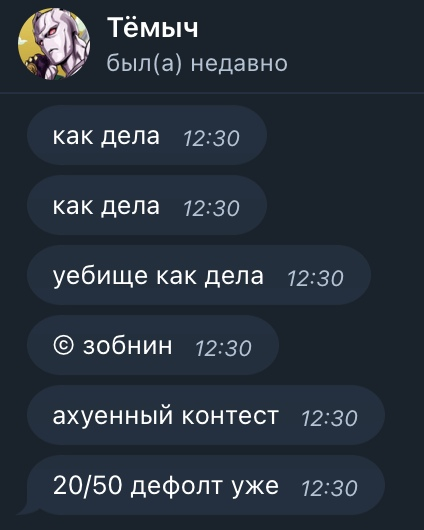
\includegraphics[scale=0.5]{3.jpg}
\end{center}
\clearpage
\section*{Номер 8}
\subsection*{a)}
\[
\int \text{arctg} x \, dx = \int 1 \cdot \text{arctg} x \, dx = 
\]
Интегрируем по частям:
\[
u' = 1
\]
\[
u = x
\]
\[
v = \text{arctg} x
\]
\[
v' = \frac{1}{1+x^2}
\]
Тогда:
\[
 = x \text{arctg} x - \int \frac{x}{1+x^2}\,dx = 
\]
Этот интеграл уже считали на семе:
\[
= x \text{arctg} x  - \frac{1}{2} \ln (1+x^2) + C\]
{\Large \begin{center}
\textbf{Ответ: } 
\[
x \text{arctg} x  - \frac{1}{2} \ln (1+x^2) + C
\]
\end{center}}
\clearpage
\subsection*{b)}
\begin{equation*}
\begin{gathered}
\int x^2 \cos^2 x \, dx = 
\end{gathered}
\end{equation*}
Интегрируем по частям:
\begin{equation*}
\begin{gathered}
u' = \cos^2 x\\
u = \int \cos^2x  \, dx = \frac{1}{2} \int (1 + \cos 2x)\, dx = \frac{x}{2} + \frac{\sin 2x}{4} \\
v = x^2 \\
v' = 2x \\
\end{gathered}
\end{equation*}
Тогда:
\begin{equation*}
\begin{gathered}
=  x^2 \left(\frac{x}{2} + \frac{\sin 2x}{4}\right) - 2 \int x \left( \frac{x}{2} + \frac{\sin 2x}{4}\right) \, dx = \left(\frac{x^3}{2} + \frac{\sin 2x \cdot x^2}{4}\right) -  \frac{2x^3}{6} - \frac{1}{2} \int \sin 2x \cdot x \, dx = 
\\
\frac{1}{2} \int \sin 2x \cdot x \, dx
\end{gathered}
\end{equation*}
Интегрируем по частям:
\begin{equation*}
\begin{gathered}
\\
f' = \sin 2x \\
f = -\frac{\cos 2x}{2}\\
g = x\\
g' = 1 \\
\\
\frac{1}{2} \left(-\frac{\cos 2x \cdot x}{2}  - \int -\frac{\cos 2x \cdot 1}{2} \, dx\right)  =- \frac{x \cdot \cos 2x}{4} + \frac{1}{4} \int \cos 2x \, dx  = \frac{x \cdot \cos 2x}{4} + \frac{\sin 2x}{8} + C
\end{gathered}
\end{equation*}
Тогда:
\begin{equation*}
\begin{gathered}
= \frac{x^3}{6} + \frac{\sin 2x \cdot x^2}{4} + \frac{x \cos 2x}{4} - \frac{\sin 2x }{8} + C
\end{gathered}
\end{equation*}
\begin{center}
{\Large \textbf{Ответ: } 
\[
\frac{x^3}{6} + \frac{\sin 2x \cdot x^2}{4} + \frac{x \cos 2x}{4} - \frac{\sin 2x }{8} + C
\]}
\end{center}
\subsection*{c)}
\[
\int \ln^2 x \, dx = 
\]
Интегрируем по частям:
\[
u' = 1
\]
\[
u = x
\]
\[
v = \ln^2 x
\]
\[
v'= \frac{2\ln x}{x}
\]
Тогда:
\[
= x \ln^2 x - 2 \cdot \int \ln x \, dx  =
\]
\[
\int \ln x \, dx = x \ln x -  \int x \cdot \frac{1}{x}\, dx = x \ln x - x
\]
\[
=  x \ln^2x - 2x \ln x + 2x + C
\]
{\Large \begin{center}
\textbf{Ответ: } 
\[
x \ln^2x - 2x \ln x + 2x + C
\]
\end{center}}
\subsection*{d)}
\[
\int x^2 \ln(1+x) \, dx 
\]
Интегрируем по частям:
\[
u' = x^2
\]
\[
u = \frac{x^3}{3}
\]
\[
v = \ln(1+x)
\]
\[
v' = \frac{1}{1+x}
\]
Тогда:
\[
\frac{x^3 \cdot \ln(1+x)}{3} - \frac{1}{3} \cdot \int \frac{x^3}{(1+x)} \, dx = 
\]
Найдем отдельно интеграл:
\[
\int \frac{x^3}{1+x} \, dx = \begin{bmatrix}
t = 1 + x \\
x = t - 1
\end{bmatrix}
=
\int \frac{(t-1)^3}{t} \, dt = \int \frac{t^3 -3t^2 +3t -1}{t} \, dt = 
\]
\[
=  \frac{t^3}{3} - \frac{3t^2}{2} + 3t - \ln(t) + C = \frac{(1+x)^3}{3} - \frac{3(1+x)^2}{2}  + 3(1+x) - \ln (1+x) + C
\]
Итого:
\[
\frac{x^3 \cdot \ln(1+x)}{3} - \frac{1}{3} \cdot \left(\frac{(1+x)^3}{3} - \frac{3(1+x)^2}{2}  + 3(1+x) - \ln (1+x)\right)  + C = 
\]
\[
=
\frac{x^3 \cdot \ln(1+x)}{3} - \frac{(1+x)^3}{9} - \frac{(1+x)^2}{2} + (1+x) - \frac{\ln(1+x)}{3} + C = 
\]
\[
= \frac{(x^3 - 1)[\ln(1+x)]}{3} - \frac{(1+x)^3}{9}  - \frac{(1+x)^2}{2}  + (1+x) + C
\]
{\Large \begin{center}
\textbf{Ответ: } 
\[
\frac{(x^3 - 1)[\ln(1+x)]}{3} - \frac{(1+x)^3}{9}  - \frac{(1+x)^2}{2}  + (1+x) + C
\]
\end{center}}
\subsection*{e)}
\[
\int \sin(\ln x) \, dx
\]
Сделаем замену:
\[
t = \ln x
\]
\[
x = e^t 
\]
\[
dx = e^t dt
\]
Тогда:
\[
\int \sin (t) e^t \, dt
\]
Интегрируем по частям:
\[
u' = e^t
\]
\[
u = e^t
\]
\[
v = \sin t
\]
\[
v' = \cos t
\]
Тогда:
\[
\int \sin (t) e^t \, dt = \sin (t) e^t - \int \cos(t) e^t \, dt
\]
Найдем интеграл отдельно:
\[
\int \cos (t)  e^t \, dt = e^t \cdot \cos (t) + \int \sin (t) e^t \, dt + C
\]
Итого:
\[
\int \sin (t) e^t \, dt = \sin (t) e^t - e^t \cdot \cos (t) - \int \sin (t) e^t \, dt + C
\]
Перенесем интеграл в левую часть:
\[
2 \int \sin (t) e^t \, dt = \sin (t) e^t- e^t \cdot \cos (t)  + C
\]
\[
\int \sin (t) e^t \, dt =\frac{ \sin (t) e^t- e^t \cdot \cos (t)}{2} + C
\]
{\Large \begin{center}
\textbf{Ответ: } 
\[
\frac{ \sin (\ln x) \cdot x -  x \cdot \cos (\ln x)}{2} + C
\]
\end{center}}
\subsection*{f)}
\[
\int \sqrt{a^2 + x^2} \, dx
\]
Интегрируем по частям:
\[
u' = 1
\]
\[
u = x
\]
\[
v = \sqrt{a^2+x^2}
\]
\[
v' = \frac{x}{\sqrt{a^2 + x^2}}
\]
Тогда:
\[
x \cdot \sqrt{a^2 + x^2} - \int \frac{x^2}{\sqrt{a^2+x^2}} \, dx
\]
Найдем интеграл:
\[
\int \frac{x^2}{\sqrt{a^2 + x^2}} \, dx = \int \frac{x^2 + a^2 - a^2}{\sqrt{a^2 + x^2}} \, dx = \int \left(\sqrt{a^2 + x^2} - \frac{a^2}{\sqrt{a^2+x^2}}\right) \, dx = 
\]
\[
=
\int \frac{x^2}{\sqrt{a^2+x^2}}\, dx - a^2 \int \frac{1}{\sqrt{x^2 + a^2}} \, dx = \int \sqrt{a^2 + x^2} \, dx - a^2 \ln (x + \sqrt{a^2 + x^2})
\]
Тогда:
\[
\int \sqrt{a^2 + x^2} \, dx = x\sqrt{a^2+ x^2} - \int \sqrt{a^2 + x^2} \, dx + a^2 \ln \left( x + \sqrt{a^2 + x^2} \right) + C
\]
Перенесем интеграл в левую часть:
\[
2 \int \sqrt{a^2 + x^2} \, dx = x \sqrt{a^2 + x^2} + a^2 \ln \left(x + \sqrt{a^2 + x^2}\right) + C
\]
\[
\int \sqrt{a^2 + x^2} \, dx = \frac{x \sqrt{a^2 + x^2}}{2}  + \frac{a^2 \ln \left(x + \sqrt{a^2 + x^2}\right)}{2}  + C
\]
{\Large \begin{center}
\textbf{Ответ: } 
\[
\frac{x \sqrt{a^2 + x^2}}{2}  + \frac{a^2 \ln \left(x + \sqrt{a^2 + x^2}\right)}{2} + C
\]
\end{center}}
\subsection*{g)}
\[
\int e^{ax} \cdot \cos (bx) \, dx 
\]
Интегрируем по частям:
\[
u' = e^{ax}
\]
\[
u = a \cdot e^{ax}
\]
\[
v = \cos(bx)
\]
\[
v' = \frac{\sin(bx)}{b}
\]
Тогда:
\[
= \frac{ e^{ax} \cdot \sin (bx)}{b} - \frac{a}{b} \int \frac{\sin (bx) \cdot e^{ax}}{1} \, dx
\]
Найдем интеграл отдельно:
\[
\int \sin (bx) \cdot e^{ax} \, dx =- \frac{e^{ax} \cdot \cos (bx)}{b} + \frac{a}{b} \int \frac{ e^{ax} \cdot \cos (bx) }{1} \, dx
\]
Тогда:
\[
\int e^{ax} \cdot \cos(bx)  \, dx  = \frac{\sin(bx) \cdot e^{ax}}{2} - \frac{a}{b} \cdot \left( - \frac{e^{ax} \cdot \cos(bx)}{b} + \frac{a}{b} \cdot \int e^{ax} \cdot \cos (bx) \, dx\right) + C = 
\]
\[
 = \frac{\sin (bx) \cdot e^{ax}}{2} + \frac{a}{b} \cdot \frac{e^{ax} \cdot \cos (bx)}{b} - \frac{a^2}{b^2} \int e^{ax} \cdot \cos (bx)\, dx + C
\]
Перенесем все налево:
\[
\int e^{ax} \cdot \cos (bx) \, dx \cdot \left(1 + \frac{a^2}{b^2} \right) = \frac{\sin (bx) \cdot e^{ax}}{2}  + \frac{a \cdot e^{ax} \cdot \cos (bx)}{b^2} + C
\]
По итогу:
\[
\int e^{ax} \cos (bx) \, dx  = \frac{\left(e^{ax} \cdot \sin(bx) \cdot b^2 + e^{ax} \cdot cos(bx) \cdot 2a \right)}{2b^2 \cdot \left(1 + \frac{a^2}{b^2}\right)} + C
\]
{\Large \begin{center}
\textbf{Ответ: } 
\[
\frac{\left(e^{ax} \cdot \sin(bx) \cdot b^2 + e^{ax} \cdot cos(bx) \cdot 2a \right)}{2b^2 \cdot \left(1 + \frac{a^2}{b^2}\right)} + C
\]
\end{center}}
\end{document}